\documentclass[12pt,twoside]{report}
\usepackage{lipsum}
\usepackage[utf8]{inputenc}
\usepackage{setspace}
\usepackage{graphicx}
\usepackage{grffile}
\usepackage{amsmath}
\usepackage{float}
\graphicspath{{images/}}
\usepackage[a4paper, width=150mm, top=25mm, bottom=25mm, bindingoffset=6mm]{geometry}
\usepackage{fancyhdr}
\usepackage[font=small,labelfont=bf]{caption}
\usepackage{listings}
\usepackage{bbm}
\usepackage{amsfonts}
\usepackage[T1]{fontenc}
\pagestyle{fancy}
\fancyhead{}
\fancyhead[RE, RO]{Data Mining for the LoRaWAN}
\fancyfoot{}
\fancyfoot[RE, RO]{\thepage} %page numbers 
\renewcommand{\headrulewidth}{0.4pt} %linewidth for header
\renewcommand{\footrulewidth}{0.4pt} %linewidth for footer
\renewcommand{\baselinestretch}{1.5}

\usepackage{biblatex}
\addbibresource{references.bib}

\usepackage[colorlinks=true,linkcolor=blue]{hyperref}

\title{Data Mining using Machine Learning algorithms on LoRaWAN data}
\author{Ante Lojić Kapetanović}
\date{September 2019}

\begin{document}

%%%%% TITLE PAGE %%%%%
\begin{titlepage}
    \begin{center}
        %\vspace*{1cm}
        
        \Large
        \textbf{UNIVERSITY OF SPLIT\\
        FACULTY OF ELECTRICAL ENGINEERING, MECHANICAL ENGINEERING AND NAVAL ARCHITECTURE}
        %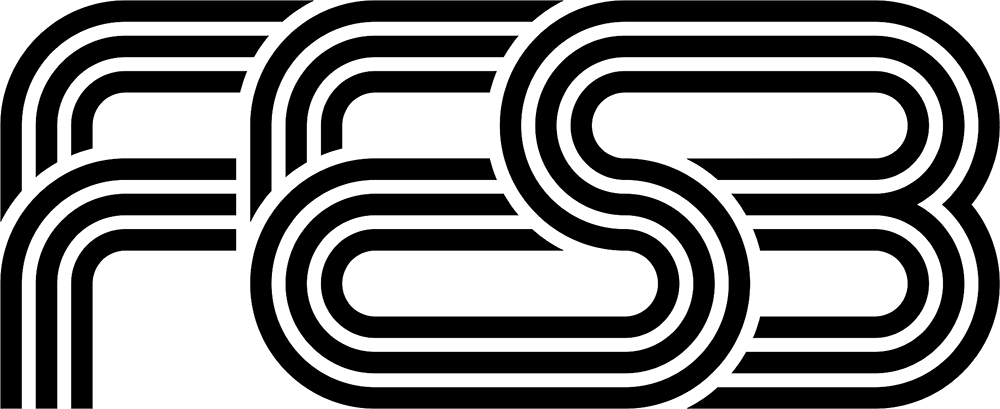
\includegraphics[width=0.2\textwidth]{fesb_logo.png}

        \vspace{4cm}

        \textbf{MASTER THESIS}

        \vspace{3cm}
        
        \Huge
        \textbf{Data Mining for the LoRaWAN}

        \vspace{5cm}

        \Large 
        \textbf{Ante Lojić Kapetanović}

        \vfill

        \large
        Split, July 2019.

    \end{center}
\end{titlepage}

\pagenumbering{roman} % start paging using roman numbers // frontmatter

%%%%% ASSIGNMENT %%%%%

\thispagestyle{plain}

{\setstretch{1.0}
\begin{figure}
  \centering
  
\includegraphics[width=1\linewidth]{assignment-header.png}
\end{figure}

Graduate study: \textbf{Electrical Engineering and Information Technology}

Program module: \textbf{Computer Engineering}

Program code: 222

Academic year: 2018./2019.

\vspace{1cm}

Name and Surname: \textbf{Ante Lojić Kapetanović}

ID-number: 750-2017

\vspace{1cm}

\begin{center}
  \textbf{\Large{Master Thesis Assignment}}
\end{center}

Title: \textbf{Data Mining for the LoRaWAN}

\vspace{1cm}

Assignment: \\Acquire knowledge on statistical models and algorithmic implementation of machine learning. 
Understanding LoRaWAN technology, its implementation and application. 
Define the measurement method and then measure the performance of LoRaWAN technology in real-time implementation. 
Collecting and cleansing measured data, then data mining and preprocessing that includes exploration analysis principles 
(define basic metrics and key performance indicators). 
LoRaWAN performance analysis using machine learning algorithms.

\vspace{1cm}

Application date: 04.03.2019.

Submission deadline: 19.09.2019.

\vspace{1cm}

Thesis submitted: 09.09.2019.

\vspace{1cm}

\begin{tabular}[b]{@{}l}
  Chairman of the\\ Examing Board:
\end{tabular}
\hfill
  Supervisor:\hspace{3cm}

\vspace{1.5cm}

\begin{tabular}[b]{@{}l}
  \textbf{prof. dr. sc. Julije Ožegović}
\end{tabular}
\hfill
  \textbf{doc. dr. sc. Petar Šolić}
}

%%%%% ACKNOWLEDGEMENETS %%%%%
\chapter*{Acknowledgements}
Firstly, I would like to start by saying big thank you to my traineeship mentors \textbf{Petar Popovski} and 
\textbf{Jimmy Jessen Nielsen}. Their office doors were always open for my research questions. Also, to all my 
colleagues from the Connectivity group of the Electrical Systems department at Aalborg University, thank you for
all enjoyable moments and help.\\

To my mentor \textbf{Petar Šolić}, who provided me with a great opportunity to connect with one of the best teams in the 
field and for giving me the freedom to shape my project the way I wanted to and for all the help during and after the research, thank you!\\

Finally, I must express my profound gratitude to my dearest family - to my mom \textbf{Divna}, my grandma \textbf{Milica}, my late uncle \textbf{Ante} and late grandpa \textbf{Josip}, and to my girl \textbf{Anja}
for providing me with unfailing support and continuous encouragement throughout my years of study and through the 
process of researching and writing  this thesis. None of this would be possible without them. Thank you.


%%%%% STATEMENT  %%%%%
\chapter*{Statement}
I confirm that the Master's thesis entitled \emph{Data Mining for the LoRaWAN} mentored by 
Petar Šolić, Ph.D. has been composed solely by myself applying knowledge, skills 
and methodology of scientific research acquired in the course of study at the Faculty 
of Electrical Engineering, Mechanical Engineering and Naval Architecture and using 
literature listed in this work. Cognitions, opinions, conclusions, mathematical 
expressions and theories cited directly or paraphrased in this thesis are referenced 
with literature sources.

\vspace{2cm}
\hspace*{\fill}Ante Lojić Kapetanović

%%%%% TABLE OF CONTENTS %%%%%

\tableofcontents


%%%%% INTRO %%%%%
\chapter{Introduction}
\pagenumbering{arabic} % start paging using arabic numbers // content
%MOTIVACIJA I ŠIRE PODRUČJE TEME RADA, ŠIRI KONTEKST, SAŽETI OPIS STANJA U PODRUČJU I VAŽNOST PODRUČJA
The Internet of Things (IoT), interconnection of computing devices embedded in everyday objects, is spreading more and more each day.
The greatest need of the IoT is the autonomy of connected devices, especially in wireless sensor networks.
Wireless sensor networks consist of energy-limited devices that ususally transmit data over long distances.
Considering the long range communication, the current trend in the IoT is the development of the protocols that enable long range coverage using low bandwidth while being as energy efficient as possible.
This thesis is concerned with the Long Range Wide Area Network (LoRaWAN) communication model and possibility of the probability assessment of future end device activation.
End devices in a LoRaWAN deployment are event driven and, as such, extremely unpredictable. 
Predicting the probability of the future end device activation can lead to avoiding collisions in the air, thus improving outage rates, throughput and, in turn, energy efficiency for persistent devices.



%SAŽETI OPIS TEME RADA (GL ELEMENTI ZADATKA, GLAVNI ELEMENTI ONOGA ŠTO JE NAPRAVLJENO U OKVIRU RADA)
%1)TEMA RADA (CCA 1 REČENICA)
%2)SADRŽAJ UVODNOG DIJELA (2-4 REČENICE)
%3)SADRŽAJ PRAKTIČNOG DIJELA RADA (2-4 REČENICE)
The main task of the thesis was to assess the nature of the end device behavior, to seek some correlations across the devices and to examine the predictability of the traffic based on the independent activations of the LoRaWAN deployment on the city lights of Svebølle, Denmark.
If the prediction is possible and could be made flawlessly for each end device, one could make a protocol without the scheduling overhead.
This new potential protocol could result in better throughput, reliability and latency.
The thesis starts with theoretical overview of the LoRaWAN, its physical layer and media access control layer as well as the communication model. 
Before the prediction model, there is a gentle introduction to a time series data, characteristic for the IoT traffic. 

%SAŽETI PRIKAZ SADRŽAJA POJEDINIH POGLAVLJA (3-5 REČENICA PO POGLAVLJU)
The chapter two is dealing with an in-depth overview of the LoRaWAN technology. 
The LoRaWAN physical layer and media access control layer are both described, along with key performance features, parameters and message frame formats.

The IoT end devices can have scheduled activity or can be event driven. 
Scheduled IoT traffic, when captured, results in a time series data where each data point is indexed in time order.
If the IoT devices are event-driven, the measured data is still structured as sequential but the period of time between time points is not equal.
A time series data and the applicable forecasting methods are explained through the chapter three. 

The first half of the forth chapter is dedicated to the network topology of the actual observed LoRaWAN deployment. 
The data preprocessing and transforming processed data set to the time series are also described.
The second half proposes the deep neural network model for predicting the future end device activation. 
The Python implementation of the model itself is in the Appendix A.
Finally, results are given in the last section of the chapter and the conclusion based on the results is given in the chapter five.

%%%%% CONTENT CHAPTERS %%%%%
\chapter{Theory behind the LoRaWAN}
%% example on how to properly add a picture
% \begin{figure}[h]
%     \centering
%     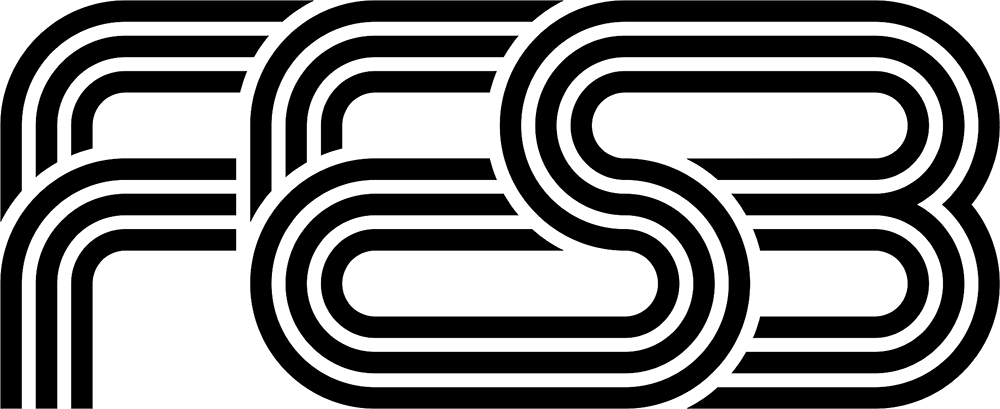
\includegraphics[scale=0.2]{fesb_logo.png}
%     \caption{An example graph}
%     \label{figure:fesb_logo}
% \end{figure}

Long Range Wide Area Network, or LoRaWAN for short, is a low power, media access control (MAC) protocol for wide area networks.
The LoRaWAN is often used in the Internet of Things (IoT) deployment, specially in a smart environment where there are thousands of end-devices (i.e. sensors) that require minimal bandwidth and consume low power.
The IoT is the extension of Internet connectivity into physical devices and everyday objects. 
The IoT, as an interconnection concept, serves, and will serve, variety of devices exchanging information about themselves and their surroundings.
Even though there are very few concrete definitons of the IoT, its classification can be defined strictly when it comes to the range. 
Three basic types of the IoT wireless networks, considering range, are:
\begin{itemize}
    \item short-range wireless IoT with commonly used communication protocols such as Bluetooth, Light-Fidelity, Near-field communication (NFC), Radio-frequency identification (RFID), Wi-Fi, ZigBee, etc.
    \item medium-range wireless IoT and the high-speed communication protocol for mobile networks LTE-Advanced
    \item long-range wireless IoT with protocols \textbf{Low-Power wide-area network} \\ (\textbf{LPWAN}) which is designed to allow long range communication at very low data rate thus reducing the power consumpiton and the overall cost of the transmission. There are a few widely used and relatively recent protocols: \textbf{LoRaWAN}, Sigfox, NB-IoT, Weigtless, RPMA.
\end{itemize}
An IoT device has limited memory, processing power and bandwidth and, most importantly, a low amount of available energy \cite{Aloys_LoRa}.
The core idea of the IoT is to maximize the lifetime of device's battery because by the end of 2020 there is expected to be over 50 bilion connected devices \cite{Evans_IoT}.
If the attitude of doing as much as possible with least amount of power consumed is taken as the most important in the IoT, it is easy to realize that standard cellular networks, as well as the WiFi technology are too \textit{power-hungry} and there is a strong need for using up-to-date technologies that fulfill the communication requirements of the IoT.

\section{LoRa technology overview}
LPWANs, unlike the traditional broadband, are not focused on enabling high data rates per device. 
Instead, the most important performance metrics are energy efficiency, scalability and coverage \cite{Mikhaylov_LoRaWAN}.

The current version of LPWAN is constructed as a cellular network consisted of the end devices (ED) and the base stations (BS). 
EDs are connected to and served by a BS thus forming a star-topology network around them, see fig. \ref{fig:lpwan}.
\begin{figure}[h]
    \centering
    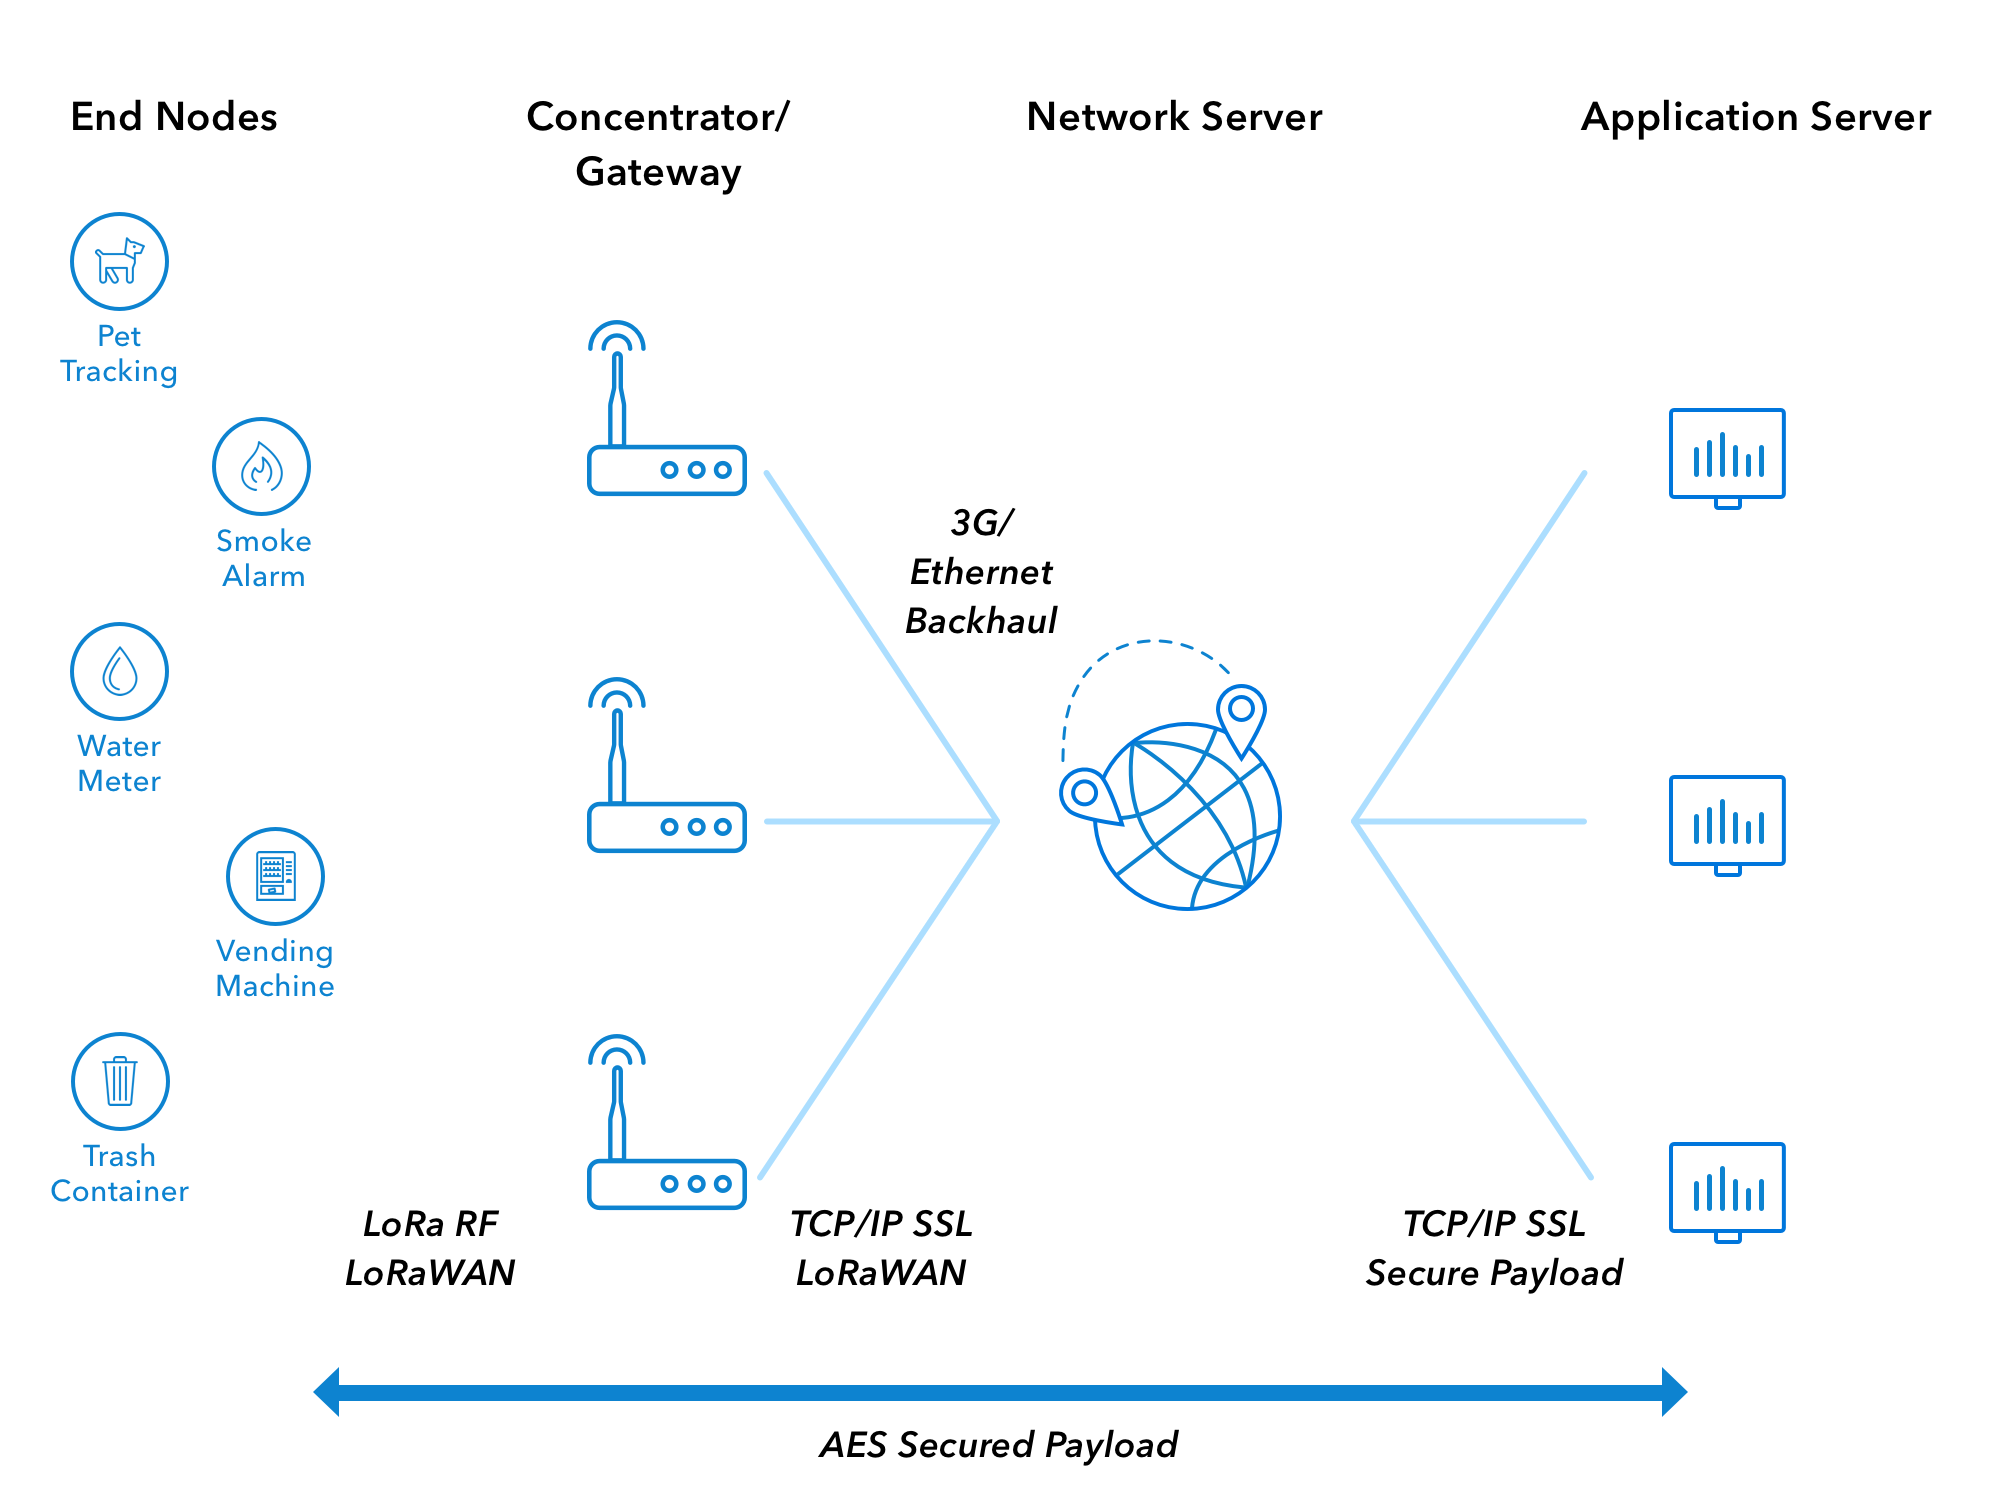
\includegraphics[width=\linewidth]{lpwan.png}
    \caption{An LPWAN as a star-of-stars topology network. Every end device is connected to a base station and every base station is connected to a central \textit{hub}, in this case to a network server \cite{TTN}.}
    \label{fig:lpwan}
\end{figure}

The most of the traffic in LPWANs is uplink where an ED communicates only to a BS and not with other EDs. A BS rarely sends any messages to an ED.

\textbf{LoRa} is the LPWAN protocol that targets deployments for already described environment (limited energy, low bandwidth, long range communication).
LoRa, as a long-range communication system, can refer to two distinct layers: \cite{Aloys_LoRa}
\begin{enumerate}
    \item a physical layer using the Chirp Spread Spectrum (CSS) modulation technique
    \item a media access control (MAC) layer protocol (LoRaWAN) 
\end{enumerate}
While the LoRaWAN is an open standard \cite{lora-alliance}, LoRa is a proprietary modulation technology based on the chirp spread spectrum developed and maintained by Semtech. 

\section{LoRa physical layer}
\subsection{Physical layer features}
The LoRa physical layer is a modulation based on the CSS scheme that uses wideband linear frequency modulated pulses whose frequency increases or decreases based on the encoded information \cite{Mikhaylov_LoRaWAN}.
Frequency offsets between the receiver and the transmitter are equivalent to timing offsets because of the linearity of the chirp and thus easily eliminated in the decoder. 
This also makes the LoRa modulation immune to the Doppler effect. 
Besides Doppler resistance, LoRa key properties are: long range connectivity, high robustness, multipath resistance, low power consumption \cite{Bor_LoRA}.

The CSS, as a modulation technique, is used to encode and transmit the data over large distances in the 868MHz band \cite{Reynders_CSS}. 
Chrip stands for Compressed High Intensity Radar Pulse and it is a signal which frequency, as mentioned, either increases (up-chirp) or decreases (down-chirp) with time.
Chirps are linear, which means that the frequency varies linearly with time:
\begin{equation}
    f(t) = f_{0} + kt
\end{equation}
where $ k $ is the slope of the chirp:
\begin{equation}
    k = \frac{f_{1} - f{0}}{T}
\end{equation}
The phase is described as:
$$ \theta (t) = \theta_{0} + 2\pi \int_{0}^{t}f(\tau)d\tau $$

$$ \theta (t) = \theta_{0} + 2\pi \int_{0}^{t}(f_{0} + kt) d\tau $$

\begin{equation}
    \theta(t) = \theta_{0} + 2\pi (f_{0}t + \frac{k}{2}t^{2})
\end{equation}
where $ \theta_{0} $ is the initial phase and $ f_{0} $ is the initial frequency.

There are several frequency bands LoRa can operate in, but the European frequeny band is defined in the 863-870 MHz range.
European regulations specify duty-cycles on devices for each sub-band.
The duty cycle indicates the fraction of time a resource is busy \cite{TTN}. 
Europen standards are defining the duty cycle at 1\% for most regions. 

\subsection{Parameters of the LoRa physical layer}
There are three key parameters for customization of the LoRa modulation:
\begin{itemize}
    \item bandwidth (BW) - the range of frequencies in the transmission band
    \item spreading factor (SF) - the ratio between the symbol rate and the chirp rate
    \item code rate (CR) - the FEC rate used by a modem to protect against the bursts and interferences
\end{itemize}
One LoRa symbol is composed of $ 2^{SF} $ chirps, which are spread all over the frequency band.
It starts with a preamble which is represented by a number of continuous up-chirps \cite{Knight}.
The last two and one forth chirps are the sync word after which the transmission of the actual payload begins, shown in fig. \ref{fig:lora_signal}.
\begin{figure}[h]
    \centering
    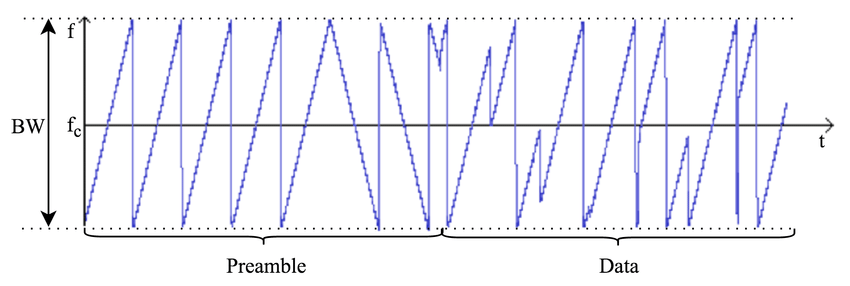
\includegraphics[width=\linewidth]{lora-signal.png}
    \caption{A frequency variation in time of a modulated signal emitted by a LoRa transmitter \cite{Aloys_LoRa}}
    \label{fig:lora_signal}
\end{figure}

As there are $ 2^{SF} $ chirps in a symbol, a symbol can effectively encode SF bits of information, where higher SF increases the signal-to-noise ratio (SNR) but also affects the air time of the packet.
From here, it is easy to derive the duration of the symbol regarding the spreading factor and the bandwidth:
\begin{equation}
    T_{s} = \frac{2^{SF}}{BW}
\end{equation}

Taking the relation of the code rate with the bandwidth and the spreading factor, and the fact that SF bits of information are transmitted per symbol, the useful bit rate is formulated with the equation:
\begin{equation}
    R_{b} = SF \times \frac{BW}{2^{SF}} \times CR 
\end{equation}

A data rate is a number of information bits that are conveyed per unit of time \cite{Silva_LoRaWAN}.
The adaptiveness should be enabled whenever the end device has stable RF conditions. 
The Adaptive Data Rate (ADR) optimizes the bit rate, the airtime and the energy consumption, and is affected mostly by the signal-to-noise ratio and the number of gateways that recevied each uplink message.

\subsection{Physical frame format}
A LoRa physical frame begins with a preamble. 
In fig. \ref{fig:lora_signal}, it is shown that the preamble starts with constant up-chirps that spread throughout the whole frequency band. The last two and one forth upchirps are the sync word which represents one byte value that is used to differentiate LoRa networks that use the same frequency band.
After the preamble, comes the optional header. The header is always configured with the code rate of 4/8.
The header indicates the size of the payload in bytes, the code rate used for the end of the transmission and wheter or not a 16-bit payload CRC is present in the frame \cite{Aloys_LoRa}.
If the information in a header is known in advance, there is no need to use a header.
The payload part of a frame is the actual data which size is limited on 255 bytes per frame.
After a payload, there is an optional cyclic redundancy checker on the end of the frame.
A frame is depicted in fig. \ref{fig:lora_phy_frame}.
\begin{figure}[h]
    \centering
    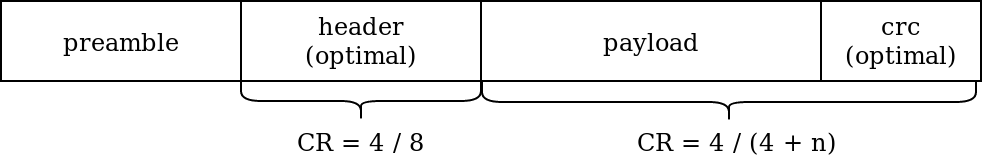
\includegraphics[width=\linewidth]{phy-frame.png}
    \caption{The structure of a LoRa frame}
    \label{fig:lora_phy_frame}
\end{figure}

The physical layer payload is consisted of elements defined in the official LoRaWAN specification from LoRa Alliance \cite{Sornin_LoRaWAN}.
The complete length of the physical layer payload is given by:
\begin{equation}
    PL = MHDR + MACPayload + MIC 
\end{equation}
where $MHDR=1$ is the length of the MAC header, $MACPayload$ is the media access control layer payload and $MIC=4$ is the message integrity code.
\begin{multline}
    PL = MHDR + FHDR_{ADDR} + FHDR_{FCTRL} +\\ FHDR_{CNT} + FHDR_{OPTS} + FPort + FRMPayload + MIC 
\end{multline}
where the payload of the MAC layer is consisted of $FHDR_{ADDR}=4$ which is the length of the ED address field of the frame header, lengths of the frame control $FHDR_{CNT}=4$ and the frame counter $FHDR_{FCTRL}=4$ fields and $FHDR_{OPTS}$, which is the length of the optional FHDR field carrying MAC commands.
$FPort=1$ is the application specific port identifier.
Taken all \textit{a priori} known lengths, the length of the physical layer payload is now:
\begin{equation}
    PL = 12 + FHDR_{OPTS} + FPORT + FRMPayload
\end{equation}

\section{Media access control layer}
\subsection{Devices and the network topology overview}
LoRaWAN is a media access control protocol built on top of LoRa and, unlike LoRa, is completely open sourced.
It is often used in the IoT deployment where end devices are simple rudimentary electronic devices with embedded sensors. 
End devices are expected to transmit packets to a base station using LoRa proprietary modulation with a low data rate using small bandwidth.
The LoRaWAN protocols are defined in \cite{Sornin_LoRaWAN}.
LoRaWAN architecture is based on a star-of-stars topology depicted in fig \ref{fig:lorawan}.
\begin{figure}[h]
    \centering
    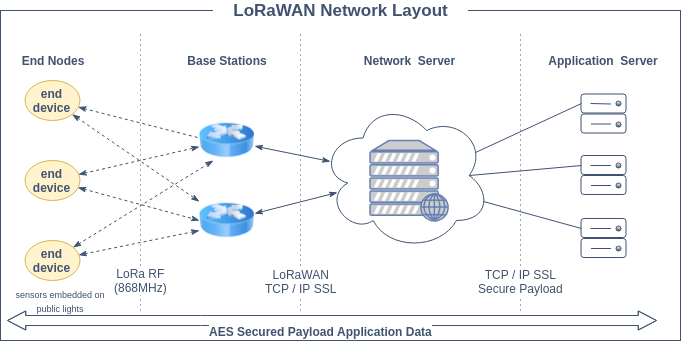
\includegraphics[width=\linewidth]{LoRaWAN-Network-Layout.png}
    \caption{Network topology of a typical LoRaWAN-based network. The communication is most often uplink, end devices send data to a base station which capture the MAC frames and dispatch them to a network server using a back-haul interface with high througput}
    \label{fig:lorawan}
\end{figure}
This architecure enables long range communication while keeping the device battery lifetime as long as possible.

There are three device types defined in the LoRaWAN specification:
\begin{description}
    \item[Class A devices] support bi-directional communication between the end device and the base station. Uplink message can be sent randomly, at any time. The end device opens two receiving windows RX1 and RX2 at specified times (1 second and 2 second respectively) after an uplink transmission. If there is no reply from the server during the duration of RX1 or RX2, the next opportunity to send data will happen after the next uplink transmission from the end device. Class A device mechanism is depicted in fig. \ref{fig:classA}.
    \item[Class B devices] extend the Class A functionality by adding scheduled receive windows for downlink traffic from the server.
    \item[Class C devices] behave similar to the Class A devices, but keep the receiving window continuosly open. They are at a high level of power consumption but achieve low-latency communication.
\end{description}
\begin{figure}[h]
    \centering
    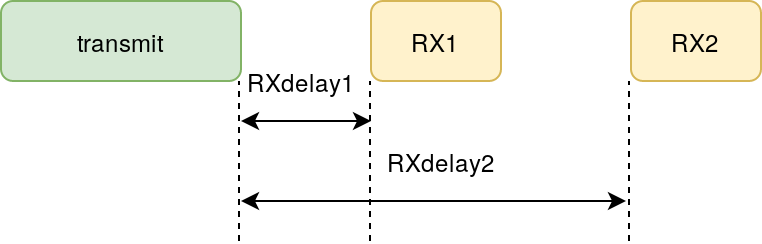
\includegraphics[width=0.7\linewidth]{classA.png}
    \caption{Class A device is commonly used device in the LoRaWAN deployment. RX1 and RX2 are receving windows enabled for server to respond but configured in a way that server should not use both RX windows}
    \label{fig:classA}
\end{figure}

LoRaWAN does not support device-to-device communication, packets can be transmitted only from an end device to a network server or, rarely, from a server to an end device.

\subsection{LoRaWAN message format}
Inside the payload section of the LoRa frame, depicted in fig. \ref{fig:lora_phy_frame} there are MAC header (MHDR), which indicates the type of MAC message, the MAC payload, which carries application data and the Message Integrity Code (MIC), which allows a receiver to check the integrity of a MAC message received.
The content of the MAC payload is the frame header (FHDR), the frame port (FPort) and the frame payload \cite{ibanez_lorawan}. 
The LoRaWAN media access control message format is shown in fig. \ref{fig:lora_mac_frame}.
\begin{figure}[h]
    \centering
    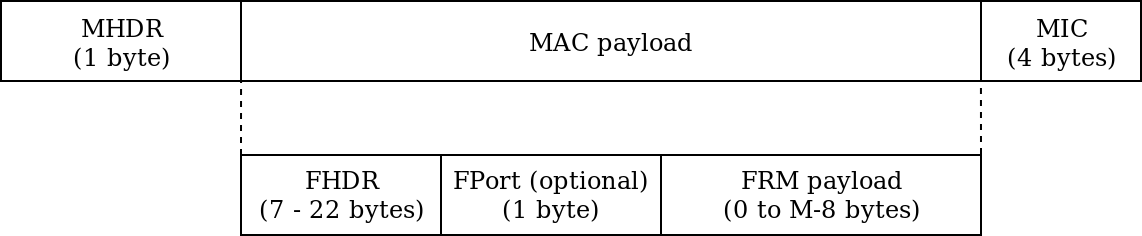
\includegraphics[width=\linewidth]{lora-mac-frame.png}
    \caption{LoRaWAN MAC message format. The FPort field is present when the frame payload field contains data (has non-zero length). $M$ is the maximum size of the MAC Payload field. The frame header (FHDR) field has a size of 7 bytes if it does not contain options, and up to 22 bytes when options are used.}
    \label{fig:lora_mac_frame}
\end{figure}

FHDR is consited of:
\begin{itemize}
    \item DevAddr -- 4 bytes end device address
    \item FCtrl -- 1 byte frame control further consisted of different flags for uplink and downlink messages
    \item FCnt -- 2 bytes frame counter
    \item FOpts -- use to piggyback MAC commands on a data message
\end{itemize}

The minimal size of the MAC header is 13 bytes while the maximal size is 28 bytes.

\subsection{Network setup and security}
To deploy a LoRaWAN network, it is important to activate end devices. 
All LoRaWAN devices have a 64 bit unique device identifier (DevEUI) that is assigned by the chip manufacturer.
Communication is done using 32 bit device address (DevAddr) where the first 7 bits are dedicated for the hosting network and 25 bits are left to be assigned to individual devices. 
The assignment of the DevAddr identifier is done through an activation procedure. 
There are two basic ways to activate the end device: \cite{TTN}
\begin{itemize}
    \item Over-The-Air Activation (OTAA) -- more secure way to connect in which devices perform a join-procedure with the network (negotiation of security keys)
    \item Activation By Personalization (ABP) -- hardcoding the DevAddr to the end device
\end{itemize}

Other than DevAddr, during the activation procedure the following information should be inquired by the end device: \cite{Aloys_LoRa}
\begin{itemize}
    \item application identifier (AppEUI) -- a global application ID that identifies the owner of the end device
    \item network session key (NwkSKey) -- a key used by the network server and the end device to verify the MIC of all data to ensure data integrity
    \item application session key (AppSKey) -- a key used by the network server and the end device to encrypt and decrypt the payload field of data messages
\end{itemize}

The extensive view on the security and the security challenges of LoRaWAN is given in \cite{security_lora}. Here, only key features and possible improvements will be presented.
The LoRaWAN utilizes two layers of security: one for the network and one for the application layer. 
The network layer security is responsible for the authenticity of the end device in the network, while the application layer security makes sure that the network operator does not have access to the actual content of the MAC payload.
The process of the end device activation is marked with secure keys exchange. 
Two session keys (NwkSKey and AppSKey) are unique to each device and to each session. 
If a device is dynamically activated via the OTAA activation, keys will be generated again with each new activation. 
If the end device is statically activated through the ABP activation process, secure keys are hardcoded and stay the same with each activation.
LoRaWAN systems come with end-to-end data confidentiality and integrity that should be manufacturer and network provider agnostic. 
The encryption with the key exchange implemented in the LoRaWAN is the Advanced Encryption Standard (AES), based on the security for IEEE 802.15.4 wireless networks.
Even though the LoRaWAN provides an end-to-end security both through the network security layer and the application security layer, there are still few weaknesses of the security features in the LoRaWAN standard.
Firstly, encrypted messages have the same length as the key. Secondly, if the session keys are compromised, security will be rendered ineffective as it would be too complex to change the AES keys on all nodes and devices. 
Moreover, the session keys (AppKey, NwkSKey and AppSKey) are a big issue. 
Lastly, identification and connection processes could be a huge weakness. 
All base stations send their personal IDs (beacons) periodically to the server. 
It is fairly easy for the attackers to obtain this ID, which can be used for overriding the base station.

\chapter{Time series data and forecasting methods}
%% example on how to properly add a picture
% \begin{figure}[h]
%     \centering
%     \includegraphics[width=\linewidth]{example.png}
%     \caption{example}
%     \label{fig:example}
% \end{figure}
End devices in the IoT deployment are often event-driven instead of periodically activated. 
That means that some predefined event has to happen in order to initiate the end device communication with the base station.
Usually, when the end device is mentioned in the context of the IoT, it is expected to have sensors embedded on it and, more importantly, to have connection with some gateway where data is going to be relayed to a network server and, subsequently, to an application server.
When data is collected on the base station it can be formed as:
\begin{description}
    \item[time series data] - a series of data points indexed in time order and taken at successive equally spaced points in time
    \item[sequential non-structured data] - the order of data matters but the period of time between time points is not equal 
\end{description}
Event-driven end devices or, more precisely, end devices that transmit data after they have been triggered by some event captured by the sensor, generate sequential data without any noticable equality in the time period between the two adjacent received data points on the base station end.
If devices are programmed to measure and transmit measured data to the base station, good practice is to keep the transmission equally spaced in time in order to create time series data set.
A time series data is of great interest because it provides possibility of applying forecasting methods by observing possible patterns in historical data. 
Time series forecasting can be termed as the process of predicting the future by understanding the past \cite{Raicharoen_timeseries}.

\section{General overview and main components of time series data}
A time series is a sequential set of data points, measured over successive time and is defined as a set of observations $x(t), t = 0, 1, 2,...$ where $t$ represents the time elapsed and $x(t)$ is treated as a random variable.
If the time series data set is consisted of only single observed variable, it is called univariate and in the case of multiple observed variables, it is termed as a multivariate time series. 
Talking about a standard time series data, there are four important components that affect the shape of a time series data. Those components are: \cite{Adhikari_timeseries}
\begin{itemize}
    \item trend - the tendency of a time series to increase, decrease or stagnate over a long period of time
    \item cyclicality - medium-term changes in a series caused by circumstances, which repeat in cycles
    \item seasonality - variations in a time series characterized by fluctuations within a observed period of time during the season
    \item irregular components - all unpredictable influences which are not regular and are not repeated in a particular pattern; there is no defined statistical technique for measuring a time series with this characteristic (random walks) \cite{timeseries}
\end{itemize}

An important part of the analysis of a time series is the selection of a suitable probability distribution for the data. There is always a strong possibility of future unpredictable behaviour of observed data if each observation $x_{t}$ is a realized value of a certain random variable $X_{t}$.

\section{Time series analysis and forecasting methods}
For statistics, econometrics, quantitative finance, meteorology, and geophysics the primary goal of a time series analysis is forecasting. 
In the context of signal processing, control engineering and communication engineering it is used for a signal detection and estimation.
In the context of data mining, pattern recognition and machine learning a time series analysis can be used for clustering, classification, query by content, anomaly detection as well as forecasting.
Whatever the application of a time series analysis is, it always has to start by reviewing data stationarity, seasonality and possible autocorrelation in the target variable.

The concept of a stationary process in its simplest definition can be defined as a stohastic process with statistical properties such as the mean and the variance independent upon time. 
Stationarity is a necessary condition for building a time series model that is useful for future forecasting. There are two types of stationary processes: 
\begin{itemize}
    \item strict stationary process - a stohastic process whose uncoditional joint probability distribution does not change when shifted in time, consequntly statistical parameters such as the mean and the variance do not change over time
    \item N'th order stationary process - a stohastic process achieved by computing differences between consecutive observations of the same non-strict stationary time series; the method of differencing can help stabilize the mean of time series by removing changes (i.e. trend and seasonality) in the level of the time series
\end{itemize}
In order to identify non-stationarity in the time series, it is important to observe autocorrelation function plot on the target variable. 
The autocorrelation function reflects how the observations in a time series are related to each other. 
The autocorrelation coeficient is well defined in the following formula:
\begin{equation}
    \rho_{k} = \frac{\gamma_{k}}{\gamma_{0}}
\end{equation}
where $\gamma_{k}$ is the autocovariance at a lag $k$ defined as:
\begin{equation}
    \gamma_{k} = Cov(x_{t}, x_{t+k}) = E[(x_{t} - \mu)(x_{t+k} - \mu)]
\end{equation}
and $\mu$ is the mean of the time series.
The atocovariance at the lag zero $\gamma_{0}$ is the variance of the time series. \cite{Adhikari_timeseries}

Another good condition is the ergodicity. 
Statistical properties of an ergodic process can be deduced from a single, sufficiently long, random sample of a process.
The reasoning is that any collection of random samples from a process must represent the average statistical properties of the entire process.

Before computational analysis of a time series data set, intensive cleansing methods should be performed. 
For standard stohastic forecasting models, a time series has to have stationarity property.
There are two widely used linear times series models: \emph{autoregression} (AR) and \emph{moving average} (MA).
Applying the mentioned two linear models on the data simultaneously, we get \emph{autoregressive moving average} (ARMA) which can be enriched with \emph{differentiation} (I) when the stationarity condition is not satisfied.
There are additional extensions to each of the mentioned models that deal with vector-valued data and are available under the heading of the multivariate time series data. 
Extensions on the AR(I)MA model are ARFIMA (autoregressive fractionally integrated moving average) and SARIMA (seasonal autoregressive integrated moving average).
Additional set of extensions of these models is available for use where the observed time series is driven by some \textit{forcing} time series. 
A distinction from the multivariate time series is that the forcing series may be deterministic, thus called exogenous.

Non-linear time series are characterized by changable variance over time (heteroskedasticity property).
For a time series data with non-linear patterns often used forecasting methods are ARCH (autoregressive conditional heteroskedasticity) and its variations GARCH (generalized ARCH), EGARCH (exponential GARCH), etc.

Applying the ARIMA model means that the time series data has no visible seasonality but is non-stationary.
The seasonal ARIMA (SARIMA) model is used for a seasonal, non-stationary time series. 
In this subsection, the basic ARIMA will be explained and visualized using the air passengers data set from \cite{timeseriespython}.
The air passengers data set is consisted of the number of airplane passengers for each month in ten-year period of time and is depicted in fig. \ref{fig:airpassengers}.
\begin{figure}[h]
    \centering
    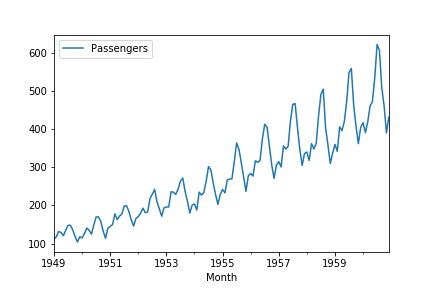
\includegraphics[width=0.7\linewidth]{airpassengers.png}
    \caption{The visualization of the exemplatory time series data: the number of passengers for each month in ten-year time period. This data is obtained from teh Github repository \cite{timeseriespython} which was used at PyCon 2017 talk on a time series analysis}
    \label{fig:airpassengers}
\end{figure}

An ARMA(p, q) model is a combination of AR(p) and MA(q) models. An AR(p) is mathematically defined as:
\begin{equation}
    y_{t} = \beta_{0} + \beta_{1}y_{t-1} + \beta_{2}y_{t-2} + ... + \beta_{n}y_{t-p} = \beta_{0} + \sum_{i=1}^{p}\beta_{i} y_{t-i}
\end{equation}
where the regression happens with past values. $\beta_{i}$ is the model parameter for value in $t-i$ moment. 
Constant $p$ represents the order of the model.

A moving average MA(q) model uses past errors as explanatory variables instead of past values of the series. The mathematical model of a moving average function is defined as:
\begin{equation}
    y_{t} = \mu + \epsilon_{t} + \sigma_{1}\epsilon_{t-1} + \sigma_{2}\epsilon_{t-2} + ... + \sigma_{n}\epsilon_{t-q} = \mu + \epsilon_{t} + \sum_{i=1}^{q}{\sigma_{i} \epsilon_{t-i}}
\end{equation}
where $\mu$ is the mean of the series, $\sigma_{i}$ is the model parameter for the $t-i$ past value moment.
The errors, $\epsilon_{i}$ where $i \in {1, 2, 3, ..., q}$ are considered as explanatory variables and $q$ is the order of the function.
A moving average model is commonly performed for curve smoothing. 

An ARMA model effectively combines an AR and a MA model and creates a general and usefull class of time series models.
Mathematically, an ARMA(p, q) is represented as:
\begin{equation}
    y_{t} = (\beta_{0} + \mu) + \epsilon_{t} + \sum_{i=1}^{p}\beta_{i} y_{t-i} +  \sum_{i=1}^{q}{\sigma_{i} \epsilon_{t-i}}
\end{equation}

Additionally, if the non-stationarity has been confirmed using the autocorrelation and/or the partial autocorrelation function (PACF), differencing should be introduced. 
The additional parameter $d$ controls the level of differencing.
In the case of the air passengers data, fig. \ref{fig:airpassengers}, differencing by $d = 1$ is depicted in fig. \ref{fig:dif}.
\begin{figure}[h]
    \centering
    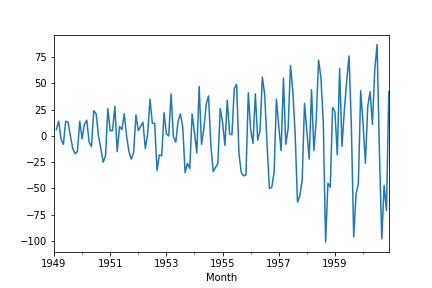
\includegraphics[width=0.7\linewidth]{dif.png}
    \caption{The order 1 differencing function performed on the air passengers data set}
    \label{fig:dif}
\end{figure}
Simple ARIMA model performed on the air passengers data is shown in fig. \ref{fig:arima}. ARIMA parameters p, d and q are configured as 2, 1, 2 respectively. 
\begin{figure}[h]
    \centering
    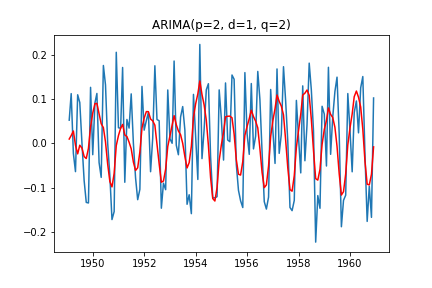
\includegraphics[width=0.7\linewidth]{arima.png}
    \caption{The ARIMA model with parameters p=2, d=1 and q=2 performed on the air passengers data set}
    \label{fig:arima}
\end{figure}

It is fairly obvious that applying described ARIMA model on observed data set is far from perfect but has potential to become strong forecasting method for the time series data when applied correctly.

\section{Introducing artificial neural networks}
Artificial neural networks (ANN) approach for time series modeling and forecasting has reached a great level of importance in the last couple of years.
ANNs are so widely used because of the powerful pattern classification and the pattern recognition cappabilities. 
Since 1940s, ANNs are developed to mimic the intelligence and the mechanism of human brain \cite{ann_history}.
Over the years ANNs have spread out to variaty of different fields such as business, industry and engineering, science, etc. because of the ability to learn from the past experience and provide inference to the output.

\subsection{The ANN architecture and common applications}
The most widely used ANNs in forecasting problems are visualized in fig. \ref{fig:ann}. 
The model has 3 layers: \emph{input layer}, \emph{hidden layer(s)} and \emph{output layer}.
The output of the model is computed using the mathematical expression: \cite{zhang_ann_ts}
\begin{equation}
    y_{t} = \alpha_{0} + \sum_{j=1}^{q}{\alpha_{j}q(\beta_{0j} + \sum_{i=1}^{p}{\beta_{ij}y_{t-1}}) + \epsilon_{t}}
\end{equation}
where $\alpha_{j}$ and $\beta_{ij}$ are the model parameters, $p$ is the number of input nodes and $q$ is the number of hidden nodes, $g$ is the transfer function at the hidden layer, $\epsilon_{t}$ is the random error and, lastly, $\alpha_{0}$ and $\beta_{0j}$ are the bias terms.
The transfer function of the hidden layer(s) for the time series data is a logistic sigmoid function, where $g(x)$ is applied as the nonlinear activation function:
\begin{equation}
    g(x) = \frac{1}{1 + \exp^{-x}}
\end{equation}
\begin{figure}[h]
    \centering
    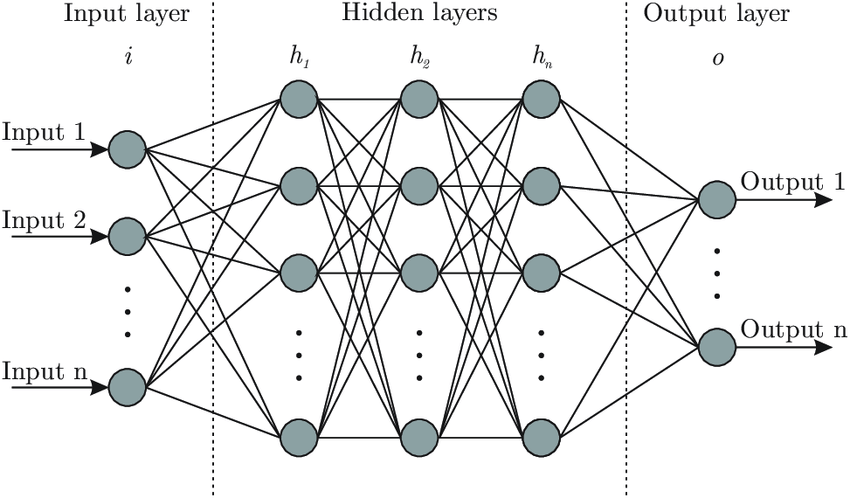
\includegraphics[width=0.8\linewidth]{ann.png}
    \caption{Common visualization of the multi-layer perceptron (MLP) neural network, which uses the hidden layer feed forward network (FNN). The figure was acquired from \cite{ann_architecture}}
    \label{fig:ann}
\end{figure}
The feed forward ANN model described above is the oldest form of the ANN where a non-linear functional mapping is performed from the past observations of the time series to the future value, $y_{t} = f(y_{t-1}, y_{t-2}, ..., y_{t-p}, \textbf{w}) + \epsilon_{t}$, where $\textbf{w}$ is a vector of all parameters and $f$ is a function determined by the network structure and connection weights \cite{Adhikari_timeseries}.

\subsection{Recurrent neural networks for the time series data}
ANNs are good predictors for the time series data because of the three main reasons:
\begin{description}
    \item[data-driven and self-adaptiveness] There is no need to make \textit{a priori} assumptions about statistical distribution of the data before feeding the ANN with the data \cite{Adhikari_timeseries}
    \item[non-linearity] ANNs are perfect for modeling data without obvious patterns  \cite{Zhang_ANN}
    \item[universial functional approximators] Any continuous function can be approximated to any accuracy \cite{Hornik_ANN}  
\end{description}

Even though \textit{vanilla} ANNs are very powerful tool to create predictions based on historical events, they do lack persistence. 
Recurrent neural networks (RNN) are solving this issue implementing loops and allowing information to persist, depcited in fig. \ref{fig:rnn}.
\begin{figure}[h]
    \centering
    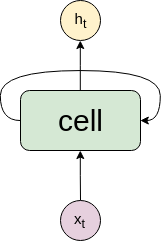
\includegraphics[width=0.2\linewidth]{RNN.png}
    \caption{The recurrent neural network is a version of the artificial neural network with loops in them, allowing the information to persist. The cell looks at the input $x_{t}$ and outputs a value $h_{t}$, while the loop allows the information to be passed from one step of the network to the next \cite{Olah_LSTM}}
    \label{fig:rnn}
\end{figure}

RNNs are using the gradient descent (first-order iterative optimization algorithm, usually used for finding the local minimum of the function) as a way to minimize the error caused by changing each weight in the proportion to the derivative of the error with the respect to that weight.
The main problem with this approach is the error gradient vanishing, which is causing the RNN to become unable to learn how to connect the information if the relevant data is devided by large gap.
The vanishing gradient problem happens when the leading eigenvalue of the weight matrix becomes too small. 
This situation can lead to gradient signal becoming so small that learning becomes extremely slow and, eventually, stops working.
The shrinkage of the gradient during the back propagation is described as:
$$ w_{t} = w_{t-1} - r * gradient $$
where $w_{t}$ and $w_{t-1}$ are weights in the current and the former iteration, and $r$ is learning rate.

The inner workings of the RNN are shown in fig. \ref{fig:rnn-unpacked}.
\begin{figure}[h]
    \centering
    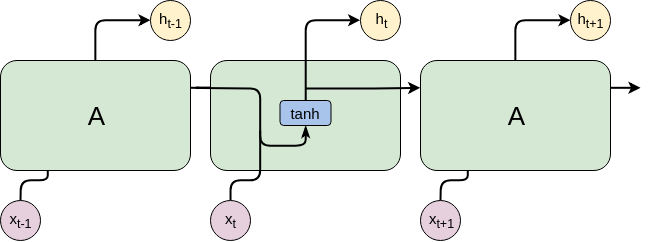
\includegraphics[width=0.8\linewidth]{RNN-unpacked.png}
    \caption{Unpacked recurrent neural network has the form of a chain of repeating cells. Each cell has its own \textit{tanh} activation function}
    \label{fig:rnn-unpacked}
\end{figure}

\subsection{Long short-term memory networks and their improvements for modeling the time series data}
Just like the RNN, long short-term memory (LSTM) network architecture is formed as a chain structure. 
The difference is that every cell has four in-layers, each performing specific operations on the input data and interacting with others in a special way. The general overview of an LSTM network is shown in fig. \ref{fig:lstm}.
\begin{figure}[h]
    \centering
    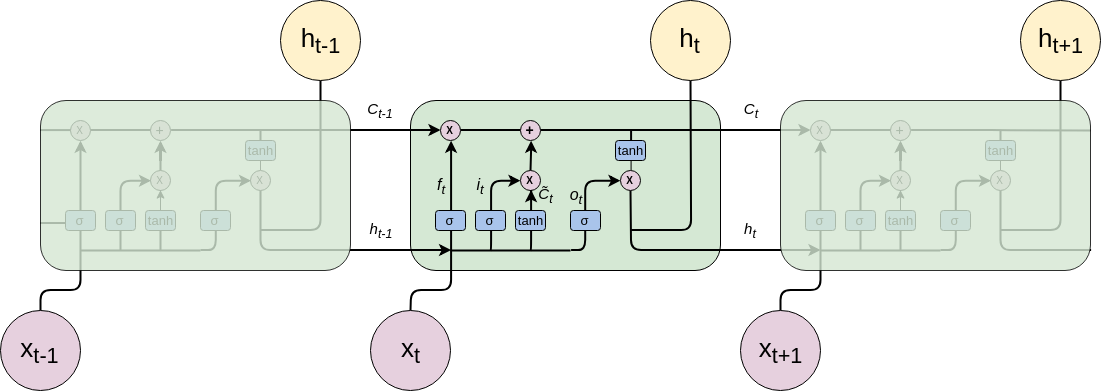
\includegraphics[width=\linewidth]{LSTM.png}
    \caption{LSTM network high-level layout. Each line carries an entire vector - from the output of one node to the input of others. All depicted algebraic operations are pointwise and blue boxes represent different activation function}
    \label{fig:lstm}
\end{figure}
Green boxes represent cells (or neurons) of the network and since the LSTM is recurrant network, both new input $x_{t}$ and the output of the previous cell $h_{t-1}$ are fed to the current cell.

An LSTM cell is consisted of five components which allow it to model both long-term and short-term data: cell state at time $t$ ($C_{t}$), hidden state ($\tilde{C}_{t}$), input gate ($i_{t}$), forget gate ($f_{t}$) and output gate ($o_{t}$).
The cell state, presented with the upper horizontal line in fig. \ref{fig:lstm},  runs through the whole cell and is affected by minor linear changes. 

Inside each LSTM cell, there are mechanisms called \emph{gates} that allow information to be passed in the selective fashion from the LSTM to the cell state. 
There are three types of gates in LSTM network:
\begin{itemize}
	\item {Forget gate} - determines which information to remove from the cell state using \textit{sigmoid} function that outputs value between 0 (completely reject) and 1 (completely accept)
		$$ f_{t} = \sigma (W_{f} \cdot [h_{t-1}, x_{t}] + b_{f}) $$
		where
		\begin{itemize}
			\item[] $ x_{t} $ is the current input vector,
			\item[] $ h_{t-1} $ is the previous cell's output value,
			\item[] $ W_{f} $ is the associated weight,
			\item[] $ b_{f} $ is the added bias.
		\end{itemize}
	\item {Input gate} - decides what new information should be written to the cell state. 
	
	Firstly, the \textit{sigmoid} function decides which value to update:
	$$ i_{t} = \sigma (W_{i} \cdot [h_{t-1}, x_{t}] + b_{i}) $$ 
	where
	\begin{itemize}
		\item[] $ x_{t} $ is the current input vector,
		\item[] $ h_{t-1} $ is the previous cell's output value,
		\item[] $ W_{i} $ is the associated weight,
		\item[] $ b_{i} $ is the added bias.
	\end{itemize}

	After that, the \emph{tanh} layer creates a vector of candidates to be added to the cell state. 
	$$ \tilde{C}_{t} = tanh (W_{C} \cdot [h_{t-1}, x_{t}] + b_{C}) $$
	where
	\begin{itemize}
		\item[] $ x_{t} $ is the current input vector,
		\item[] $ h_{t-1} $ is the previous cell's output value,
		\item[] $ W_{C} $ is the associated weight,
		\item[] $ b_{C} $ is the added bias.
	\end{itemize}
	\item {Output gate} - decides what is going to be the output of the concrete cell. 
	$$ o_{t} = \theta (W_{o} [h_{t-1}, x_{t}] + b_{o}) $$ 
	where
	\begin{itemize}
		\item[] $ x_{t} $ is the current input vector,
		\item[] $ h_{t-1} $ is the previous cell's output value,
		\item[] $ W_{o} $ is the associated weight,
		\item[] $ b_{o} $ is the added bias.
	\end{itemize}
	
	The output is based on the filtered version of the cell state.
	$$ h_{t} = o_{t} \times tanh(C_{t})$$
	where 
	$ C_{t} $ is the new cell state calclulated as:
	$ C_{t} = f_{t} \times C_{t-1} + i_{t} \times \tilde{C}_{t} $
\end{itemize}

An LSTM network is a huge step up considering a RNN. 
The LSTM architecture is proposed in 1997 in \cite{Hochreiter_LSTM} and it found its application in many fields that deal with sequenced data forms.
For this thesis, a LSTM is of the special interest because it is a good fit for a time series data. 



\chapter{Proposed end device activity prediction LSTM model and results}
%% example on how to properly add a picture
% \begin{figure}[h]
%     \centering
%     \includegraphics[width=\linewidth]{example.png}
%     \caption{example}
%     \label{fig:example}
% \end{figure}

% %  example on how to properly add a code snippet
% \begin{lstlisting}[language=Python]
%     <insert code here>
% \end{lstlisting}
    
    

The core idea behind this thesis is to apply forecasting methods on the data from the real LoRaWAN deployment in Svebølle, Denmark.
Throughout this chapter, topology of the network as well as the communication model of the network will be explained.
Also, data processing, cleaning and transforming methods prior to the modeling are explained. 
The idea of modeling the transformed data is to examine whether there is a possibility of predicting future activation of event-driven end devices.
The activation of the end device is characterized as a successful uplink data transmission and proposed model for predicting is LSTM, an artificial recurrent neural network architecture widely used in the field of deep learning on sequential data.

The reasons for the activity prediction are diverse but knowing the probability of activation for given future time interval can help a great deal in the battery life savings.
There are usually thousands of devices connected in the single IoT network and improving energy efficiency is important research topic to deal with. 
One example the improving of the battery life for this deployment could be strategic positioning of the end device regards to the base station. 
Placing the base station near the devices that are more likely to transmit data could lead to decrease of the package time-on-air (ToA).


\section{Network topology of the deployment in Svebølle, Denmark}
As previosly defined, the LoRaWAN topology is a star-of-stars type where each end device is connected and transmit data to the base station (or multiple stations) and the base station is connected via higher bandwidth protocol to the network server.
The network server decodes the packets received from the base station and after performing security checks transmits data to theapplication server.
The application server is usually hosted on cloud infrastructure platforms such as Google Cloud, Amazon Web Server or Azure.

This thesis uses data measurued on the base station end of the LoRaWAN network deployment in Svebølle, Denmark. 
End devices are set on city lights and there is a single base station, network deployment in fig. \ref{fig:svebolle}.
\begin{figure}[h]
    \centering
    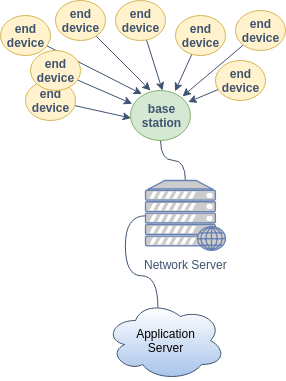
\includegraphics[width=0.5\linewidth]{Svebolle-Topology.png}
    \caption{Overview of the network topology of the LoRaWAN deployment on city lights in Svebølle}
    \label{fig:svebolle}
\end{figure}
Atmospheric data is collected and sent sporadically to the base station.
Base station collected the data with the encrypted MAC payload where relevant attributes are:
\begin{itemize}
    \item \textit{time} - in datetime format to microsecond precision
    \item \textit{DevAddr} - end device public 32-bit address wirten in HEX format
    \item \textit{freq} - radio frequency of the carrier signal
    \item \textit{chan} - used channel
    \item \textit{BW} - bandwidth
    \item \textit{SPF} - spreading factor
    \item \textit{RSSI} - received signal strength indication
    \item \textit{SNR} - signal-to-noise ratio
    \item \textit{CR} - code rate
    \item \textit{DR} - data rate
    \item \textit{CRCstatus} - flag that indicates if there were transmission error
    \item \textit{mType} - type of MAC message
    \item \textit{MACPayload} - the actual, intended message in encrypted form
\end{itemize}

The communication model is depicted in fig. \ref{fig:sv_cm}.
\begin{figure}[h]
    \centering
    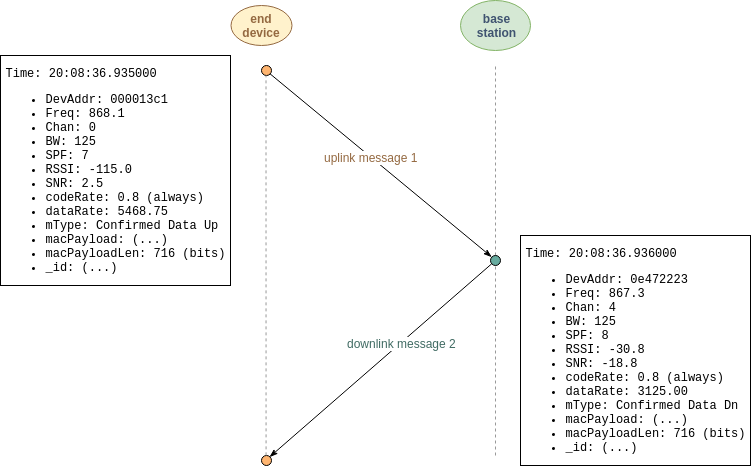
\includegraphics[width=\linewidth]{Svebolle-ed-bs-model.png}
    \caption{Two-way communication model between the end device and the base station in the LoRaWAN deployment in Svebølle. Due to the nature of communication, end devices can be classified as Class A devices which support bi-directional communication between a device and a base station}
    \label{fig:sv_cm}
\end{figure}
Uplink messages (messages sent by an end device to the base station) can be sent at any time and there is no regular pattern in uplink transmissions. 
Downlink messages happen when devices open receiving windows at specified times (1s and 2s) after an uplink transmission.
If there is no response from the server, the next opportunity will be after the next uplink transmission from an end device.

\section{Measured data}
The measurement took place during a five month period where about six hundred thousand data points were captured on the base station end.
The data set contains 250 unique device addresses where there is large disproportion between the number of transmission for each device. 
The data known prior to transmission is device address, frequency of the carrier signal, channel, bandwidth, spreading factor, code rate and message type as well as MAC payload.
On the receiver end (base station) RSSI and SNR are captured.
Statistical inference, the process of deducing properties of an underlying probability distribution, is shown in fig. \ref{fig:fit}. 
\begin{figure}[h]
    \centering
    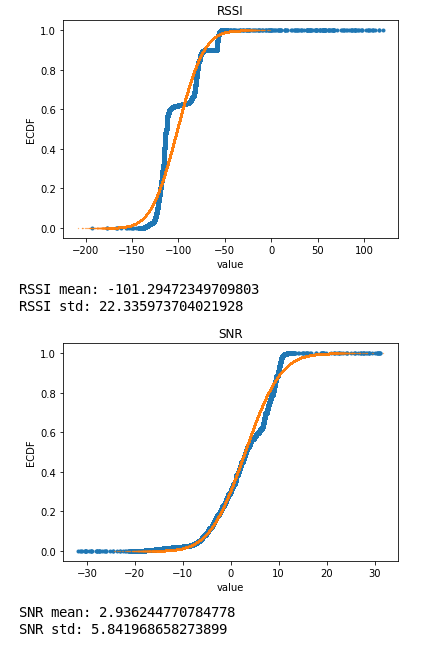
\includegraphics[width=0.6\linewidth]{fit.png}
    \caption{RSSI and SNR value distribution in comparisson to theoretical Rician distribution. Blue dotted plot represents the actual measured data, while orange line represents the Rician theoretical distribution}
    \label{fig:fit}
\end{figure}
We use statistical inference to make probabilistic conclusions about what can be expected if the data is collected again.
If the theoretical distribution is fitting the measured data, we will be able to draw acceptable conclusions from the data and give more general conclusions from relatively few data points.
In fig. \ref{fig:fit}, there is a comparisson between the actual distribution and the Rice theoretical distribution but due to the high irregularity in the measured data, it doesn't make a perfect fit.


\section{Data preprocessing and transformation to a time series format}
Due to the nature of the problem of the future activation prediction for each end device, many of the captured attributes are irrelevant.
The measurements in the data set are not structured as a time series data, only moments when transmission of LoRa messages were successful in uplink direction were captured and stored.
Since time series data is a series of data points indexed in time order and taken at successive equally spaced points in time, the data set had to be processed.
The only important label in the processed data set is the flag which indicates wheter the end device sucessfully transmitted the message to the base station or not.
For each time point, where every time point is observation in seconds, there is an activity flag assigned.
If the device was active for observed time point, the activity flag is 1, otherwise the activity flag is 0.
Since the measurements were carried out through long period, newly created data set was large enough to be suitable candidate for applying deep learning methods to perform forecasting of future time points.

Above described process was carried out using Python 3.7.1 programming language using following methods:
\begin{itemize}
    \item extracting the only important features from the data set, \textit{Time} of the event and \textit{DevAddr}, which stands for 32-bit public end device address. The data set was preloaded into the data frame, two-dimensional size-mutable, potentially heterogenous tabular data structure with labeled axes \cite{df} .
    \begin{lstlisting}[language=Python]
        def get_features(df):
            return df[['Time', 'DevAddr']]
    \end{lstlisting}
    \item lowering time resolution from nanosecond precision to second precision, which means if input is 2017-01-02 12:08:27.788000, output will be 2017-01-02 12:08:27.
    \begin{lstlisting}[language=Python]
        def clean_features(df):
            Time = list(df.Time.values)
            Time_parsed = []
            sep = '.'
            for t in Time:
                t_parsed = t.split(sep, 1)[0]
                Time_parsed.append(t_parsed)
            df.Time = Time_parsed
            df['Time'] = pd.to_datetime(df['Time'])
            return df
    \end{lstlisting}
    \item selecting the device whose activity will be predicted
    \begin{lstlisting}[language=Python]
        def select_dev(df, dev_name='000013c1'):
            df = df[df.DevAddr == dev_name]
            df = df.reset_index(drop=True)
            df = df.Time
            df = df.drop_duplicates(keep='last')
            df = pd.DataFrame({'Time':df.values})
            return df
    \end{lstlisting}
    \item adding activaty flag 1
    \begin{lstlisting}[language=Python]
        def add_label(df):
            df['Active'] = 1
            return df
    \end{lstlisting}
    \item resampling data in order to achieve the time series format. For each second there is either flag 0 or 1 which indicates the device activity.
    \begin{lstlisting}[language=Python]
        def datetime_resampling(df):
            df = df.set_index('Time')
            df.index = pd.to_datetime(df.index)
            df = df.resample('1S').asfreq()
            df = df.fillna(0)
            return df
    \end{lstlisting}
\end{itemize}

Post-processed data set was stored in the data frame data structure with only two columns, one for the datetime and the other for the end device activation indicator.

\section{Proposed LSTM model for predicting future activation of end devices}
The LSTM model was developed using Keras, a high-level neural networks API, capable of running on top of Tensorflow.
Tensorflow is an open source software library for numerical computation using data flow graphs.
The graph nodes represent mathematical operations, while the graph edges represent the multidimensional data arrays (tensors) that flow between them \cite{tensorflow}.

The workflow of the neural network development is particulary well suited and fine-tuned for large-scale machine learning.
Its basic principle is very simple: first a graph of computations in Python has to be defined and then Tensorflow takes that graph and runs it efficiently using optimized C++ code \cite{Aurelian}.

Tensorflow allows the user to break up the graph into several chunks and run them in parrallel across many CPUs and GPUs.
Also, it supports distributed computing for creating and training large neural networks on the big data.

The created graph is shown in fig. \ref{fig:graph} and is described in detail in \autoref{chap:appendix}.
\begin{figure}[H]
    \centering
    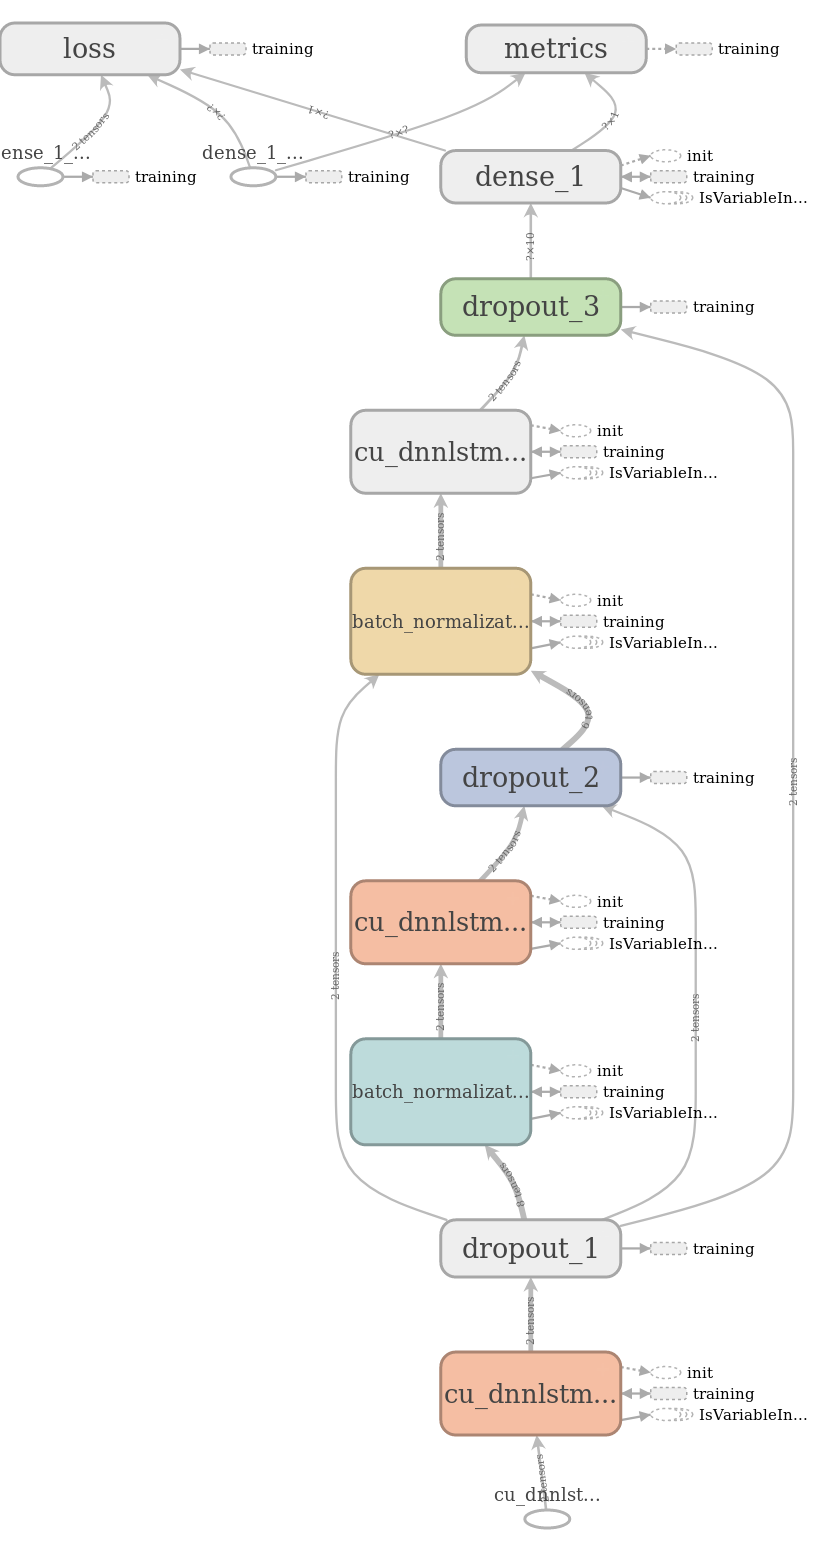
\includegraphics[width=0.7\linewidth]{graph.png}
    \caption{The dataflow graph representing the LSTM model created to predict the future end device activation using the large dataset described through the last chapter.
    The dataflow graph is used to represent the computation in terms of the dependencies between individual operations}
    \label{fig:graph}
\end{figure}
The Adam (Adaptive Moment Estimation) optimizer is used.
The Adam optimization algorithm is an extension to the stohastic gradient descent and it combines the best properties of AdaGrad and RMSProp algorithms to provide an optimization that can handle sparse gradients on noisy problems.

In order to implement the LSTM neural network, it is important to create the sequential network model.
The sequential model allows simultaneously taking a sequence of inputs and produce a sequence of outputs.
The data set is further processed to be able to fed the network.
From the processed time series data, time-delayed time series data is created using specific \textit{window size}.
If the window size is $n$, for every time point sequence of $n$ historical values will be created.
That means the activation of the current time point $y(t)$ is conditioned by the activation in moments $y(t-1), y(t-2), ..., y(t-n)$.
The following function shows how the time-delayed data set is created. $X$ is an array of sequences that each has $delay$ historical elements, while the $y$ is the array of elements that succeeds each of the respective sequnces from the $X$ array.
\begin{lstlisting}[language=Python]
    def timeDelay(df, delay):
        X_data, y_data = [], []
        
        for i in range(delay, len(df)):
            X_data.append(df[i-delay: i].tolist())
        X_data = np.array(X_data)
        y_data = df[delay:]
        return np.reshape(X_data, (X_data.shape[0],\
                                   X_data.shape[1], 1)),\
               np.reshape(y_data, (len(y_data), ))
\end{lstlisting}
This sequential model contains multiple layers of memory cells, thus creating a deep LSTM network.
After each LSTM layer, the dropout layer is applied. 

Dropout layers are added in order to prevent overfitting the training set, common issue for deep sequential neural networks.
Dropout was proposed in \cite{dropout} in 2012 and it has proven to be highly successful.
The dropout algorithm is a fairly simple one: at every training step, every neuron (including the input neurons but excluding the output neurons) has a probability $p$ of being temporarily \textit{dropped out}, meaning it will be entirely ignored during this training step, but it may be active during the next step. 
The hyperparameter $p$ is called the \textit{dropout rate}. 
After training session, neurons don't get dropped anymore \cite{Aurelian}.

The LSTM layer was realized as CuDNNLSTM, which is a fast LSTM implementation backed by cuDNN and can only be run on GPU.
The NVIDIA CUDA Deep Neural Network library (cdDNN) is a GPU-accelerated library of primitives for DNNs. cuDNN provides highly tuned implementations for standard routines such as back propagation, pooling, normalization and activation layers.
The first LSTM layer contains 128 neurons with added return sequnce, which returns the last output.
After the LSTM layer and the dropout layer comes batch normalization. 
Batch normalization normalizes the output of a previous activation layer by subtracting the batch mean and dividing by the batch standard deviation where batch is hardcoded to the value of 64.
The batch size defines the number of samples that will be propagated through the network.
The second layer is again represented as follows: the LSTM layer, dropout, batch normalization.
The last layer contains a small size LSTM layer with 10 neurons and without return sequence. 
Then again, droput is applied. 
Finally, the last part of the last layer is the dense single-neuron layer which performs multiplying the input value and the weight, adds a bias and activates the result.
The output is, in this case, a value between 0 and 1 for each input sequnce. 

The training process starts with all weights initialized randomly. 
During the training, random weights are changing due to some neural network performance metrics. 
Usually, this performance metrics is observed in terms of loss function. 
Loss function is a function that defines accuracy for trained network and should be much lower in the end of the training.
Thus, the problem of training is equivalent to the problem of minimizing the loss function. 
This model has the MSE (mean square error) function implemented and training was done through 10 epochs where each epoch is one forward pass and one backward pass of all training examples.

\section{Results}
\subsection{Output interpretation}
The described LSTM model is usually used for the time series where each time point on x-axis has some value attached to the y-axis. 
In terms of machine learning, this model is best for the regression problem where the concrete value of the future moment will be predicted.
Mainly, an LSTM network is used in the natural language processing (NLP), weather forecasting, stock predictions or any basic regression task applied to the time series data. 
For this data set, the problem is more of a classification nature than it is a regression task. 
We want to create the predictions of the activation for each end device in the LoRaWAN deployment where the activation is a \textit{bool} value that indicates if the transmission is going to happen (1) or not (0).

After the training process, the validation on the test set was done.
The data set of sequnces created using \textit{timeDelayed} function was split on the train and the set in the 80:20 ratio using the following function:
\begin{lstlisting}[language=Python]
    def split(X, y, ratio):    
        test_split = int(len(X) * ratio)
        
        X_train, y_train = X[:test_split], y[:test_split]
        X_test, y_test = X[test_split:], y[test_split:]
        return X_train, y_train, X_test, y_test
\end{lstlisting}
Since the last layer is a single-neuron dense layer with linear activation function, the output was not defined as binary output (classification) but rather as any value from 0 to 1.
For the described model trained in 10 epochs with the time delay of 5 historical values, the output was the following array (considering only a single device, with no multivariate analysis):
\begin{lstlisting}[language=Python]
    array([[1.21673493e-05, 5.82448400e+06],
           [1.52176805e-03, 2.00000000e+01],
           [1.84416212e-03, 2.00000000e+01],
           [1.91396230e-03, 2.00000000e+01],
           [1.91468524e-03, 2.00000000e+01],
           [1.91875699e-03, 2.00000000e+01]])
\end{lstlisting}
There is an obvious difference between those values and the interpretation was done using the following code:
\begin{lstlisting}[language=Python]
    y_test_pred_10[y_test_pred_10==1.21673493e-05]=0
    y_test_pred_10[y_test_pred_10!=0]=1
\end{lstlisting}
In fig. \ref{fig:output}, the predicted data after the interpretation and the actual data of the test set are depicted.
\begin{figure}[h]
    \centering
    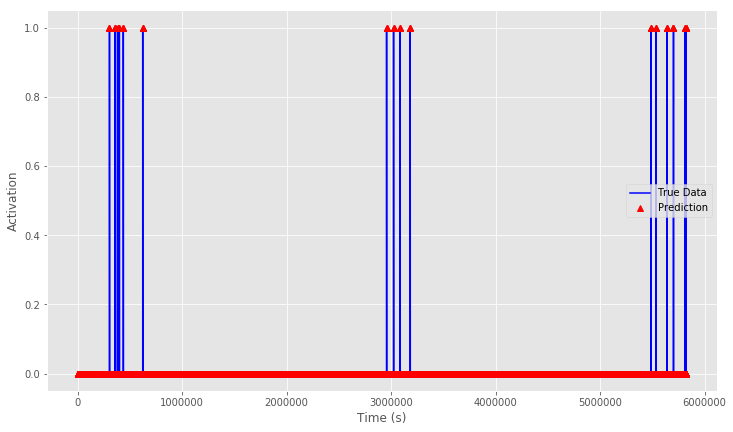
\includegraphics[width=\linewidth]{output.png}
    \caption{The processed LSTM output is represented with red triangles, which estimate moments in which observed device is active (1) or not active (0), while blue lines represent the actual device activation}
    \label{fig:output}
\end{figure}

Since this problem cannot be considered classification nor regression, it is hard to define the error metric.
The idea was to determine how far the predicted data is from the actual value in seconds.
In most cases it is 1 to 5 seconds but the worst case scenario is depicted in fig. \ref{fig:err}.
\begin{figure}[h]
    \centering
    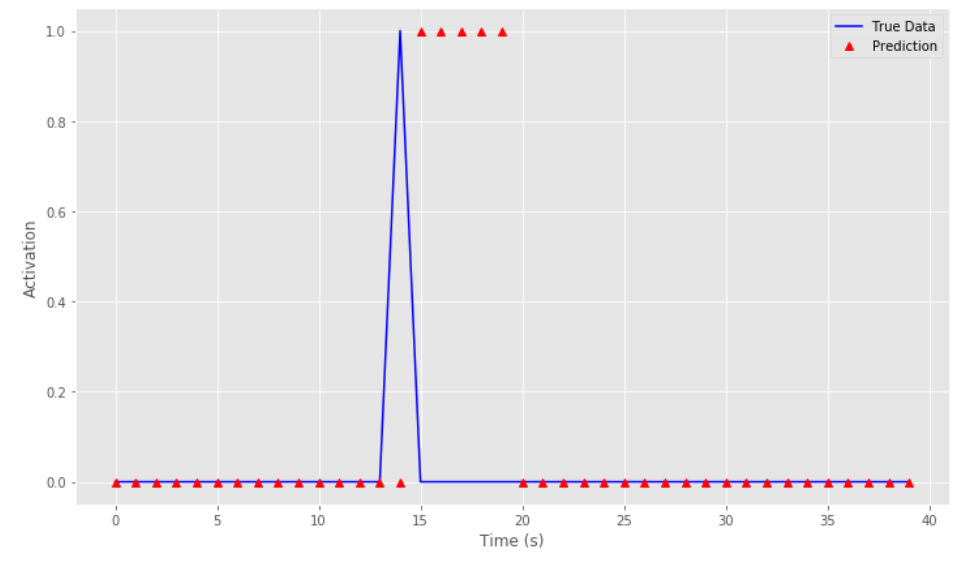
\includegraphics[width=\linewidth]{err.png}
    \caption{Error predictions for some time points not only miss the moment of the actual activation but also they are multiplied by the number of the delay initialized in the process of creating the time-delayed time series data set for training}
    \label{fig:err}
\end{figure}
For some events network predicts activation very close to the actual activation but multiplies number of events by the number of delay performed in the creation of time-delayed data set, in this case by 5.

The root mean square error (RMSE) between moments of the actual activation versus the predicted activation is a bit below 2s.
To put the RMSE rate in context, the RMSE value is compared to time difference between two activations.
In fig. \ref{fig:err_con}, the histogram of time differences is shown.
The vertical line represents the RMSE value.
If the occasional multiplication of predicted activations is ignored, the histogram could be a good error indicator.
The left area of the histogram is the percentage of mispredicted activations, while the right area of the histogram is the percentage of correctly predicted end device activations. 
The percentage of mispredicted activations (the error percentage) is 0.35\%.

\begin{figure}[H]
    \centering
    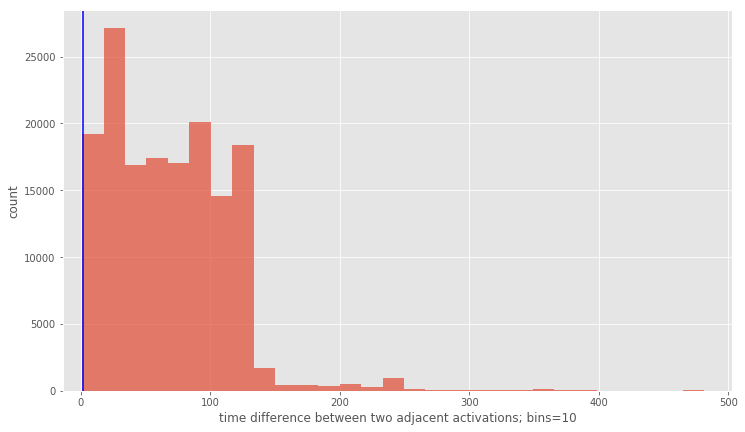
\includegraphics[width=\linewidth]{err_con.png}
    \caption{Histogram of time differences for each two adjacent end device activations}
    \label{fig:err_con}
\end{figure}

\subsection{Probability estimation of activation of the end device in a future arbitrarily-large time interval}
The core idea of the thesis is not to be able to create accurate predictions for a single point, but rather to create the probability estimation of the end device activation in a future time interval.
The general hypothesis is defined as follows: for the given period of time ($n$ seconds), the probability of the end device activation (transmission of the LoRa uplink message) should rise up as a time period gets bigger.
$$ n = 0 \Rightarrow p_{a} = 0 $$
$$ n \in <0, +\infty> \Rightarrow p_{a} \in <0, 1> $$
$$ n = \infty \Rightarrow p_{a} = 1 $$
where $n$ is the number of seconds of the future time interval for which the probability of an end device activation, $p_{a}$, will be calculated.

The algorithm for calculating the probability of the end device activation based on predicted data set is defined in the following code:
\begin{lstlisting}[language=Python]
    def estimate_prob(data, window_size):
        windows = gen_window(data, n=window_size)

        window_prob = []

        for window in windows:
            ones_freq = 0
            for data_point in window:
                if data_point == 1:
                    ones_freq += 1
            window_prob.append(ones_freq/window_size)
        return 1 - window_prob.count(0.0)/len(window_prob)
\end{lstlisting}
where the function takes two parameters, the predicted and processed output of the LSTM model as \textit{data} and the arbitrarily sized time window (number of seconds) as \textit{window\_size} for which the estimation of the probability of the end device activation will be calculated.
Considering the size of the window, \textit{windows} list is generated using the function \textit{gen\_window} which yields a sliding window over data from the iterable sequnce of data. 
The \textit{gen\_window} function:
\begin{lstlisting}[language=Python]
    def gen_window(seq, n):
        it = iter(seq)
        result = tuple(islice(it, n))
        if len(result) == n:
            yield result
        for elem in it:
            result = result[1:] + (elem,)
            yield result
\end{lstlisting}
For each \textit{window} in the list of \textit{windows} the number of activation is counted and the probability of the activation is calculated.
The final prediction is calculated as the mean of activation probabilites for each time window.
In fig. \ref{fig:prob}, it is shown how the probability of the end device activation based on the predicted data set is increasing with time.
\begin{figure}[h]
    \centering
    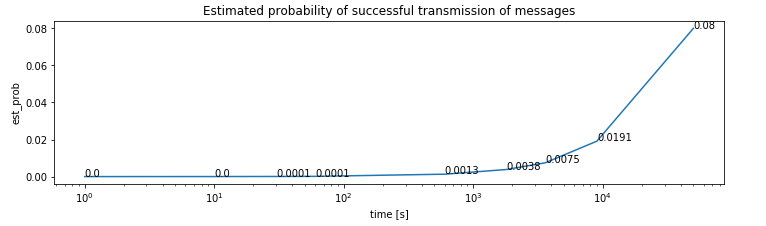
\includegraphics[width=\linewidth]{est-prob.png}
    \caption{The estimation of the probability of a single end device activation on the test data}
    \label{fig:prob}
\end{figure}

%%%%% CONCLUSION %%%%%
\chapter{Conclusion}
% SAŽETI PRIKAZ MOTIVACIJE ZA RAD U ŠIREM PODRUČJU TEME 
Through this thesis, the prediction model for the end device activation in the Long Range Wide Area Network (LoRaWAN) was proposed.
The LoRaWAN has recently emerged as an open sourced media access control protocol built on top of proprietary physical layer, LoRa, employing the CSS modulation technique.
The LoRaWAN is used for low power wide area networks (LPWAN) where the power efficient communication over very long distances is required.
These kind of networks are deployed for wireless sensor networks, where the activation of an end device is triggered with an event.
Without the scheduling on the base station of a network, collisions occur incessantly.  
This causes retransmissions and, consequently, a significantly greater energy consumption.
With the possibility of the end device activation predicition, communication protocols could be upgraded, but since there is a low chance of the prediction working in the stohastic environment, alternative forecasting methods had to be introduced.

% TEMA RADA, GLAVNI ELEMENTI ONOGA ŠTO JE NAPRAVLJENO
%1. TEMA RADA (1 REČENICA)
%2. SADRŽAJ UVODNOG DIJELA (2-4 REČENICE)
%3. SADRŽAJ PRAKTIČNOG DIJELA (2-4 REČENICE)
The Long Short-Term Memory (LSTM) neural network prediction model was developed and trained on the time series data set from the real LoRaWAN deplyment. 
An overview of the LoRaWAN technology and forecasting methods for a time series data were investigated during the theoretical part of the thesis. 
The LSTM model was created using Python programming language and Keras neural-network library, which runs on top of TensorFlow GPU. 

% SAŽETI PRIKAZ OSTVARENIH REZULTATA, VLASTITI ZAKLJUČCI TEMELJEM OSTVARENIH REZ
% OPCI ZAKLJUCCI O PRIMJENJENOM I REALIZIRANOM SUSTAVU I METODI
The predictive, sequntial model (implementation in \autoref{chap:appendix}) had been trained on the large time series data set where only the activation of the observed device for specific moment was captured.
Output values for each input sequence of historical data varied from 0 to 1.
Closer the value is to 0, there is a smaller chance that the actual activation for the future moment will happen.
Root mean square error (RMSE), considering time distance between the actual and the predicted event, was less than 2s.
The real problem is multiplied predicted activation for some moments, where instead of single activation, multiple activation is predicted.
In fig. \ref{fig:prob}, it is shown that the probability of an end device activation for the observed future time period raises as the time period raises.

Even though the results look promising, there are a few issues.
Firstly, only data from a single device was observed. 
In a wireless sensor network there are hundreds and more of devices, which means that creating data and training multiple models for each device would be extremely slow and exhausting.
Moreover, this model is adjusted for univariate time series data and as such, correlations with other devices are not taken into account. 
Lastly, becuase of the hardware limitation, the model was trained using 10-second sequences of historical data. 
Longer training sequences would not only improve the model itself, but also output could be sequnce predictions insted of point-to-point predictions.

%%%%% BIBLIOGRAPHY %%%%%
\printbibliography
\addcontentsline{toc}{chapter}{Bibliography}


%%%%% FIGURES LIST %%%%%
\listoffigures
\addcontentsline{toc}{chapter}{\listfigurename}

%%%%% ABSTRACT %%%%%
\chapter*{Summary}
\addcontentsline{toc}{chapter}{Summary} 
\thispagestyle{plain}
\begin{center}       
    \large
    \vspace{0.9cm}
    \textbf{Data Mining for the LoRaWAN}
        
    \vspace{0.4cm}
    by \textbf{Ante Lojić Kapetanović}
    
\end{center}
The state of the art Internet of Things (IoT) networks are characterized with the long range connectivity, high robustness, energy efficiency and scalability as key performance properties.
The Long Range Wide Area Network (LoRaWAN) is the media access control (MAC) protocol for wide area networks designed to perfectly fit the mentioned needs. 
The LoRaWAN allows long range communication at a very low data rate thus reducing the power consumption, which is the primary goal of a modern IoT deployment.
This thesis explores the predicability of the IoT traffic which is assumed to be based on independent and unpredictable activations of devices.
The information about the probability of the end device activation for near future would result in tremendous progress: more efficient access protocols could be designed, which would subsequently result in a better throughput, reliability, latency, and also energy efficiency.
Firstly, most of the theoretical aspects of the LoRaWAN are covered in the introductory part of the thesis.
The structuring of the measured data in a time series format and the proposal of the predictive method follows.
The Long Short Term Memory (LSTM) neural network model is proposed as a way to predict the end device activations.
Finally, based on the predictive model results, the estimation of the probability of the end device activations is shown.
The discussion of the results and the application of the prediction model, along with potential improvements of the model itself, are presented in the conclusion.\\

\textbf{Keywords:} IoT, LoRaWAN, time series, LSTM


\chapter*{Sažetak}
\addcontentsline{toc}{chapter}{Sažetak} 
\thispagestyle{plain}
\begin{center}       
    \large
    \vspace{0.9cm}
    \textbf{Rudarenje podataka LoRaWAN mreže}
        
    \vspace{0.4cm}
    autor: \textbf{Ante Lojić Kapetanović}
    
\end{center}
Posljednja dostignuća i ključna svojstva Internet stvari (IoT) mreža su dalekosežno povezivanje uređaja, robustnost, energetska učinkovitost i skalabilnost mreže.
Dalekosežna mreža širokog područja (LoRaWAN) je definirana kao protokol kontrole pristupa mediju (MAC) za mreže širokog područja i dizajnirana je tako da zadovoljava navedena ključna svojstva.
LoRaWAN mreža osigurava dalekosežnu komunikaciju pri niskoj brzini prijenosa podataka, smanjujući tako potrošnju energije što je osnovni cilj modernih implementacija IoT mreža.
Ovaj rad se bavi mogućnošću predviđanja ponašanja IoT mrežnog prometa, koji se temelji na komunikaciji neovisnih i nepredvidljivih krajnjih uređaja.
Predikcijom aktivnosti krajnjih uređaja za blisku budućnost, osigurala bi se mogućnost definiranja učinkovitijih pristupnih protokola, što bi posljedično rezultiralo boljom mrežnom propusnošću i pouzdanošću same mreže ali i energetskom efikasnošću.
Kroz uvodni dio rada opisani su teoretski aspekti LoRaWAN mreže. 
Nakon toga je definirana struktura snimanog mrežnog prometa, pretvorba u vremensku seriju i prijedlog prediktivnog modela.
Prediktivni model za predviđanje aktivnosti krajnjih uređaja je sekvencijalna LSTM neuralna mreža.
Konačno, temeljem izlaznih podataka korištene neuralne mreže, procjena vjerojatnosti aktivnosti krajnjih uređaja promatrane mreže je prikazana u posljednjem dijelu rada.
Diskusija i interpretacija rezultata, kao i moguća primjena razvijenog prediktivnog modela te njegove mane su prezentirane u zaključku.\\

\textbf{Ključne riječi:} IoT, LoRaWAN, vremenske serije, LSTM


%%%%% APPENDIX %%%%%
\appendix
\chapter{Prediction model in detail}
\label{chap:appendix}
{\setstretch{1}
\begin{lstlisting}[ language=Python,
                    tabsize=4,
                    showspaces=false,
                    showstringspaces=false,
                    numbers=left,
                    numberstyle=\footnotesize,
                    basicstyle=\small,
                    breaklines=true,
                    postbreak=\mbox{\textcolor{red}{$\hookrightarrow$}\space},]
class Model():
def __init__(self):
    self.model = Sequential()

def build_model(self, configs):
    timer = Timer()
    timer.start()

    for layer in configs['model']['layers']:
        neurons = layer['neurons'] if 'neurons' in layer else None
        dropout_rate = layer['rate'] if 'rate' in layer else None
        activation = layer['activation'] if 'activation' in layer else None
        return_seq = layer['return_seq'] if 'return_seq' in layer else None
        input_timesteps = layer['input_timesteps'] if 'input_timesteps' in layer else None
        input_dim = layer['input_dim'] if 'input_dim' in layer else None
        
        if layer['type'] == 'dense':
            self.model.add(Dense(neurons, activation=activation))
        if layer['type'] == 'lstm':
            self.model.add(CuDNNLSTM(neurons, input_shape=(input_timesteps, input_dim), return_sequences=return_seq))
        if layer['type'] == 'dropout':
            self.model.add(Dropout(dropout_rate))
        if layer['type'] == 'BatchNormalization':
            self.model.add(BatchNormalization())
            
    self.model.compile(loss=configs['model']['loss'], 
                        optimizer=configs['model']['optimizer'],
                        metrics=['accuracy'])

    print('MODEL Compiled')
    timer.stop()   

def train(self, X, y, epochs, batch_size, save_dir, logs):
    timer = Timer() 
    timer.start()
    print('MODEL Training Started')
    print(f'MODEL {epochs} epochs, {batch_size} batch size')

    save_fname = os.path.join(save_dir, f'{dt.datetime.now().strftime("%d%m%Y-%H%M%S")}-e{epochs}.h5')

    callbacks = [
        EarlyStopping(monitor='val_loss', patience=2),
        ModelCheckpoint(filepath=save_fname, monitor='val_loss', save_best_only=True),
        TensorBoard(log_dir=f'{logs}/{dt.datetime.now().strftime("%d%m%Y-%H%M%S")}-e{epochs}')
    ]  

    self.model.fit(X, y, epochs=epochs, batch_size=batch_size, callbacks=callbacks, shuffle=False)
    self.model.save(save_fname)

    print(f'MODEL Training Completed. Model saved as {save_fname}')
    timer.stop()

def train_generator(self, data_gen, epochs, batch_size, steps_per_epoch, save_dir):
    timer = Timer()
    timer.start()
    print('MODEL Out-of-Memory Training Started')
    print(f'MODEL {epochs} epochs, {batch_size} batch size, {steps_per_epoch} batches per epoch')
    
    save_fname = os.path.join(save_dir, '%s-e%s.h5' % (dt.datetime.now().strftime('%d%m%Y-%H%M%S'), str(epochs)))
    
    callbacks = [
        ModelCheckpoint(filepath=save_fname, monitor='loss', save_best_only=True)
    ]
    
    self.model.fit_generator(data_gen, steps_per_epoch=steps_per_epoch, epochs=epochs, callbacks=callbacks, workers=1)
    
    print(f'MODEL Out-of-Memory Training Completed. Model saved as {save_fname}')
    timer.stop()

def predict(self, x):
    print('MODEL Predicting Point-by-Point:')
    predicted = self.model.predict(x)
    predicted = np.reshape(predicted, (predicted.size,))
    return predicted
\end{lstlisting}
}

\end{document}
